\documentclass[aspectratio=169,xcolor=dvipsnames]{beamer}
\makeatletter
\def\input@path{{../../common/slides/theme/}{common/slides/theme/}{theme/}}
\makeatother
\usetheme{CleanEasy}
\usepackage[utf8]{inputenc}
\usepackage{lmodern}
\usepackage[T1]{fontenc}
\usepackage{fix-cm}
\usepackage{amsmath}
\usepackage{mathtools}
\usepackage{listings}
\usepackage{xcolor}
\usepackage{hyperref}
\usepackage{graphicx}
\graphicspath{{../../common/slides/assets/}{common/slides/assets/}{./}}
\usepackage{booktabs}
\usepackage{tikz}
\usetikzlibrary{positioning, shapes, arrows, calc, decorations.pathreplacing, arrows.meta, backgrounds, patterns, overlay-beamer-styles, angles, quotes, intersections}
\usepackage{etoolbox}
\usepackage{animate}

\lstset{
  basicstyle=\ttfamily\small,
  keywordstyle=\color{blue},
  commentstyle=\color{green!60!black},
  stringstyle=\color{red},
  showstringspaces=false,
  breaklines=true,
  frame=single,
  rulecolor=\color{black!30},
  backgroundcolor=\color{black!5},
  numbers=left,
  numberstyle=\tiny\color{black!70},
  numbersep=5pt
}

%----------------------------------------------------------------------------------------
%    TITLE PAGE
%----------------------------------------------------------------------------------------

\title[Block Meeting]{January Block Meeting}

\author[IA Math Team]{IA Math Team}

\vspace{-2cm}\date{Jan. 28, 2026}
%---------------------------------------------------------------------------------------

\begin{document}

\begin{frame}[t]
  \titlepage
\end{frame}

\begin{frame}[t]{Competitions}
We have some upcoming competitions. Please sign up!!
\vspace{1cm}
\begin{enumerate}
    \item Floyd County - 2/21
    \item Georgia Tech Math Day - 3/7 (Sign-ups CLOSED — Mr. Pomerance will sign up)
    \item Westminster Math Competition - 3/14
    % \item GCTM Varsity State 4/18
\end{enumerate}

\end{frame}

\begin{frame}[t]{T-Shirts}

\begin{figure}[ht]
    \centering
    \begin{minipage}{0.45\linewidth}
        \centering
        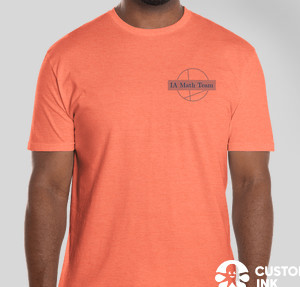
\includegraphics[width=0.8\linewidth]{frontnew.png}
        \label{new}
    \end{minipage}\hfill
    \begin{minipage}{0.45\linewidth}
        \centering
        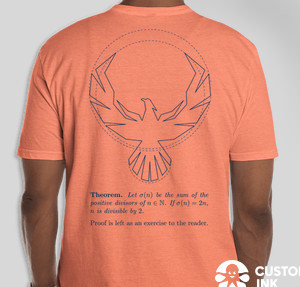
\includegraphics[width=0.8\linewidth]{backnew.png}
        \label{back}
    \end{minipage}
\end{figure}


\end{frame}

\end{document}